
%%%  یک نمونه پروپوزال کارشناسی ارشد، نسخه 0.4
%%%  وحید دامن‌افشان، دانشگاه تبریز،       http://www.damanafshan.ir
%%%   آپدیت شده در تیرماه ۹۱
%توضیحات مربوط به هر بسته یا دستور را می‌توانید در خط بالای آن ببینید.

\documentclass[12pt,a4paper]{article}
%در ورژن جدید زی‌پرشین برای تایپ متن‌های ریاضی، این سه بسته، حتماً باید فراخوانی شود
\usepackage{amsthm,amssymb,amsmath}

%دستوری برای وارد کردن واژه‌نامه انگلیسی به فارسی
\newcommand\persiangloss[2]{#1\dotfill\lr{#2}\\}
%بسته‌ای برای تنطیم حاشیه‌های بالا، پایین، چپ و راست صفحه
%\usepackage[top=30mm, bottom=30mm, left=30mm, right=30mm]{geometry}
%بسته‌ای برای نمایش تصاویر قرار داده شده در متن
\usepackage{graphicx}
% بسته‌ و دستوراتی برای ایجاد لینک‌های رنگی با امکان جهش
\usepackage[pagebackref=false,colorlinks,linkcolor=blue,citecolor=magenta]{hyperref}
% چنانچه قصد پرینت گرفتن نوشته خود را دارید، خط بالا را غیرفعال و  از دستور زیر استفاده کنید چون در صورت استفاده از دستور زیر‌‌، 
% لینک‌ها به رنگ سیاه ظاهر خواهند شد و برای پرینت گرفتن، مناسب‌تر خواهد بود.
%\usepackage[pagebackref=false]{hyperref}
%بسته‌ای برای ظاهر شدن «مراجع»  در فهرست مطالب
\usepackage{tocbibind}
%فراخوانی بسته زی‌پرشین و دستورات مربوط به نوع فونت‌ها
\usepackage{xepersian}
%تغییرات نخ
%%% ------- اضافه شده توسط نخ ------
%%% دستوری برای پنهان کردن چیزی از فهرست
\newcommand{\nocontentsline}[3]{}
\newcommand{\tocless}[2]{\bgroup\let\addcontentsline=\nocontentsline#1{#2}\egroup}

\usepackage[bottom]{footmisc}
\usepackage{indentfirst}


\settextfont{B Nazanin}
% وارد کردن دستور بالا الزامی نیست؛ چون در صورت وارد نکردن آن، فونت پیش‌فرض به صورت خودکار، فراخوانی می‌شود.
% چنانچه می‌خواهید که اعداد داخل فرمول‌ها، فارسی باشد، دستور زیر را فعال کنید
%\setdigitfont{Times New Roman}


%%%%%%%%%%%%%%%%%%%%%%%%%%%%%%%%%%%%%%%%%%%%%%%%%%%
% تعریف قلم‌های فارسی و انگلیسی برای استفاده در بعضی از قسمت‌های متن
\defpersianfont\titr[Scale=1]{B Titr}
\defpersianfont\nastaliq[Scale=1.5]{IranNastaliq}
\defpersianfont\traffic[Scale=1]{B Traffic}
\defpersianfont\yekan[Scale=1]{B Yekan}
\DefaultMathsDigits
%اگر فونت‌های بالا را ندارید، دو خط بالا را غیر فعال و دو خط زیر را فعال کنید
%\defpersianfont\traffic[Scale=1]{XB Roya}
%\defpersianfont\yekan[Scale=1]{XB Kayhan}
%%%%%%%%%%%%%%%%%%%%%%%%%%%%%%%%%%%%%%%%%%%%%%%%%%%
% تعریف و نحوه ظاهر شدن قضایا، لم‌ها، تعریف‌ها و ...
\theoremstyle{definition}
\newtheorem{definition}{تعریف}[section]
\theoremstyle{theorem}
\newtheorem{theorem}[definition]{قضیه}
\newtheorem{lemma}[definition]{لم}
\newtheorem{proposition}[definition]{گزاره}
\newtheorem{corollary}[definition]{نتیجه}
\newtheorem{remark}[definition]{ملاحظه}
\theoremstyle{definition}
\newtheorem{example}[definition]{مثال}
%%%%%%%%%%%%%%%%%%%%%%%%%%%%%%%%%%%%%%%%%%%%%%%%%%%
\begin{document}
% دستوری جهت حذف کردن شماره صفحه و سربرگ، در صورت وجود (فقط در صفحه جاری)
\thispagestyle{empty}
\vspace*{-28mm}
% نحوه درج کردن لوگوی دانشگاه
\centerline{
\includegraphics[height=5cm]{logo.png}}
\begin{center}
%دستوری برای کم کردن فاصله بین لوگو و خط پایین آن
\vspace{-2mm}
{\large \titr
گروه مستقل مهندسی رباتیک
%دستوری برای تعیین فاصله بین دو خط
\\[2.1cm]
}

{\Large \titr
تمرین پنجم درس بینایی ماشین
\\[2cm]
استاد درس:
\\[.5cm]
دکتر صفابخش
\\[1.5cm]
\large 
تدریس‌یار: 
\\[0.5cm]
مهندس مجد
\\[1.5cm]
نام دانشجو:
\\[.5cm]
نوید خزاعی
\\[.5cm]
۹۲۱۳۵۰۰۸
\\[1.5cm]
}
%دستوری برای تعیین فاصله بین خطوط (نه دو خط) و تا وقتی که مقدار آن تغییر نکند، فاصله بین خطوط، همین مقدار است.
\baselineskip=1cm

{\large
تیر ۱۳۹۳
}
\end{center}
%دستوری برای رفتن به صفحه جدید
\newpage
\pagenumbering{Alph}
\baselineskip=1cm
%دستوری برای ظاهر شدن فهرست مطالب
\tableofcontents

\baselineskip=.75cm
\newpage 
\pagenumbering{arabic}
\section{بخش اول}
%\cite{alvarez}
\subsection{روش‌های ارایه‌ی اشکال}


\textbf{پرسش:}
 در درس روش های متعددی برای ارایه اشکال توضیح داده شد. از بین این روش ها کدام یک از آن ها توسط \lr{OpenCV} پیاده سازی شده اند؟ چه روش های دیگری در \lr{OpenCV} برای ارایه اشکال پیشنهاد شده است؟
 

\textbf{پاسخ:}
از روش‌هایی که در درس مربوطه آمده‌اند، روش‌های زیر 
در 
\lr{OpenCV}

پیاده‌سازی شده‌اند: 
\begin{itemize}
\renewcommand{\labelitemi}{$\bullet$}
\item 
کد زنجیره‌ای فری‌من\LTRfootnote{ Freeman Chain Code}: 
برای محاسبه‌ی آن، لازم است پیرامون شی را داشته باشیم که در تمرینات قبلی، چگونگی به‌دست آوردن آن توسط کانتورها را دیدیم. 


\lr{CvSeq* cvApproxChains(CvSeq* src\_seq, CvMemStorage* storage, int method=CV\_CHAIN\_APPROX\_SIMPLE, double parameter=0, int minimal\_perimeter=0, int recursive=0 )}


\begin{itemize}
\renewcommand{\labelitemii}{$\circ$}
\item
\lr{src\_sec} : 
اشاره‌گری به زنجیره‌ی فریمن ورودی است که می‌تواند به زنجیره‌های دیگری نیز اشاره‌کند. در اصل باید کانتور یافت‌شده از شکل را به عنوان ورودی بدهیم. 

راه دیگری نیز پیاده‌سازی شده‌است که نیازی به این تابع ندارد و فقط با تابع پیدا کردن کانتورها، کد را ارائه می‌دهد. دقت کنید که باید در فراخوانی تابع پیداکردن کانتورها به‌ این شکل عمل کنیم:

\lr{cvFindContours(image, storage, (CvSeq**)\&chain, sizeof(*chain), CV\_RETR\_LIST, CV\_CHAIN\_CODE);}

که کانتور خروجی \lr{chain} را که از نوع 
\lr{CvChain*}
تعریف شده‌است، به نوع مناسب برای استفاده در تابع
\lr{cvFindContours}
 تبدیل کنیم. همچنین روش محاسبه‌ی کانتور باید با مقدار 
\lr{CV\_CHAIN\_CODE}
مشخص شود تا خروجی یک کد زنجیره‌ی فریمن باشد. روش نمایش این کد در حل قسمت بعدی از همین تمرین پیاده‌سازی و ارایه شده‌است.

\item
\lr{storage} : 
فضای لازم برای ذخیره‌سازی موقت محاسبات مربوط به خطوط.

\item
\lr{method} :‌
روش تخمین که مانند پارامتری با همین نام در تابع 
\lr{cvFindContours}
است و در تمرینات قبلی توضیح‌داده شده‌است. 
\item
\lr{parameter} :‌
این آرگومان مورد استفاده قرار نگرفته‌است.

\item
\lr{minimal\_perimeter} :‌
مشخص می‌کند کانتورهایی که محیطشان از این اندازه کم‌تر است، دخالت‌ داده‌نشوند.

\item
\lr{recursive} :‌
در صورت یک بودن، به صورت بازگشتی تمام کانتورهای سلسله‌مراتبی را نیز محاسبه می‌کند. در غیر این صورت کانتور اولیه‌ی بیرونی انتخاب می‌شود.

\end{itemize}

\item
توصیف‌گرهای فوریه (تبدیل فوریه‌ی گسسته): 


{\small \lr{void dft(InputArray src, OutputArray dst, int flags=0, int nonzeroRows=0)}}


\begin{itemize}
\renewcommand{\labelitemii}{$\circ$}
\item
\lr{src} : 
آرایه‌ی ورودی.
\item
\lr{dst} : 
آرایه‌ی خروجی.

\item
\lr{flags} : 

\begin{itemize}
\renewcommand{\labelitemiii}{$\diamond$}
\item
\lr{DFT\_INVERSE} : 
 به‌جای تبدیل معمولی که رو به جلو است، تبدیل معکوس فوریه را حساب می‌کند.

\item
\lr{DFT\_SCALE} :
مقیاس‌بندی جواب نهایی را مشخص می‌کند، به این ترتیب که حاصل‌ را بر طول آرایه تقسیم می‌کند.

\item
\lr{DFT\_ROWS} :
برای هر سطر از ورودی، تبدیل را جداگانه حساب می‌کند (برای کم‌کردن سربار محاسباتی در تبدیل‌های سه‌بعدی و بیشتر کاربرد دارد).

\item
\lr{DFT\_COMPLEX\_OUTPUT} :
درصورت استفاده از این پرچم، پردازش بر روی ورودی حقیقی انجام خواهد شد و خروجی با اندازه‌ی اصلی و جواب‌های مختلط خواهد بود. در حالت عادی این آرایه، به اندازه‌ی ورودی درخواهد آمد و شامل جواب‌های حقیقی است.
\item
\lr{DFT\_REAL\_OUTPUT} : 
تبدیل معکوس بر روی ورودی مختلط انجام می‌دهد. در حالت عادی جواب آرایه‌ای با اندازه‌ی ورودی و جواب‌های مختلط خواهد بود. در صورت استفاده از این پرچم حاصل به صورت حقیقی محاسبه خواهدشد. 
\end{itemize}

\item
\lr{nonzeroRows} : 
وقتی صفر نیست، تابع فرض می‌کند تنها این تعداد سطر غیرصفر از ورودی (در صورت اعمال نکردن پرچم 
\lr{DFT\_INVERSE}
) یا این تعداد از سطرهای غیرصفر خروجی (در صورت اعمال کردن پرچم 
\lr{DFT\_INVERSE}
) 
شامل عناصر غیر صفر هستند و به‌این‌ترتیب، در محاسبه‌ی بقیه‌ی سطرها صرفه‌جویی می‌شود. این پرچم برای محاسبه‌ی همبستگی متقابل\LTRfootnote{cross-correlation} 
و یا محاسبه‌ی کانولوشن با تبدیل فوریه کاربرد دارد.

\end{itemize}

\item
گشتاورهای آماری: 
برای محاسبه‌ی این ویژگی‌ها، از تابع زیر استفاده می‌کنیم:

\begin{flushleft}
\lr{Moments moments(InputArray array, bool binaryImage=false)}
\end{flushleft}


\begin{itemize}
\renewcommand{\labelitemii}{$\circ$}
\item
\lr{array} : 
آرایه‌ی ورودی، تک کاناله و هشت بیتی یا دوبعدیِ ممیز شناور. 

\item
\lr{binaryImage} : 
اگر درست باشد، تمام مقادیر غیر صفر، یک در نظر گرفته‌می‌شوند. این گزینه فقط در صورتی اعمال خواهد شد که ورودی تصویر باشد. 
\end{itemize}
خروجی از جنس \lr{Moments} می‌باشد که کلاسی شامل گشتاورهای شکل تا درجه‌ی سوم است. این کلاس سه نوع گشتاور را در خود ذخیره می‌کند: گشتاورهای فضایی\LTRfootnote{ Spatial moments}، گشتاورهای مرکزی\LTRfootnote{ Central moments}، و گشتاورهای مرکزی نرمال‌شده. 

\item
گشتاورهای هو\LTRfootnote{ Hu Moments}\cite{Hu}: 

\begin{flushleft}
\lr{void HuMoments(const Moments\& m, OutputArray hu)}
\end{flushleft}
یا

\begin{flushleft}
\lr{void HuMoments(const Moments\& moments, double hu[7])}
\end{flushleft}

که گشتاورهای آماری شکل را دریافت می‌کند و هفت گشتاور معرفی‌شده در \cite{Hu} را محاسبه می‌کند و در آرایه‌ی خروجی \lr{hu} قرار می‌دهد.

\item
اسکلت:‌ در بخش دوم به طور مفصل بر روی روش‌های پیاده‌سازی‌شده برای استخراج اسکلت شکل بحث خواهد شد.

\item
بهترین برازش بیضی: 
\begin{flushleft}
\lr{RotatedRect fitEllipse(InputArray points)}
\end{flushleft}
این روش، آرایه‌ی ورودی شامل تعدادی نقاط را دریافت می‌کند و بهترین بیضی را به آن برازش می‌کند. نتیجه در قالب یک مسطتیل دوران‌‌داده شده که بیضی در آن محیط می‌شود، محاسبه می‌شود. 



\item
بهترین برازش دایره: 

\lr{void minEnclosingCircle(InputArray points, Point2f\& center, float\& radius)}


نقاط را دریافت می‌کند و مرکز و شعاع را در دو آرگومان مربوطه قرار می‌دهد. 


\item
بهترین برازش مستطیل:
 
\begin{flushleft}
\lr{RotatedRect minAreaRect(InputArray points)}
\end{flushleft}
به نقاط ورودی، بهترین مسطیل را برازش می‌کند.

همچنین تابع

\begin{flushleft}
\lr{Rect boundingRect(InputArray points)}
\end{flushleft}

مسطتیل محاط بر شکل را می‌دهد.

\end{itemize}


همچنین می‌توان به کمک توابع پیاده‌سازی‌ شده برای پیداکردن کانتورها، خواص هندسی مانند محیط، مساحت (به کمک تابع 
\lr{contourArea}
)، عدد اویلر (تعداد سطح کانتورهای تودرتو) و گریز از مرکز\LTRfootnote{ Eccentricity} (درازی) را نیز مستقیما به دست‌آورد. این مشخصات در کلاس دربردارنده‌ی کانتور به عنوان ویژگی‌های کانتور محاسبه می‌شوند. 

علاوه بر روش‌های فوق که در درس آمده‌اند، روش‌های دیگری نیز پیاده‌سازی شده‌اند که در زیر آورده‌ شده‌اند. 

\begin{itemize}
\renewcommand{\labelitemi}{$\bullet$}
\item
برازش خم چندجمله‌ای :‌

\lr{void approxPolyDP(InputArray curve, OutputArray approxCurve, double epsilon, bool closed)}

\begin{itemize}
\renewcommand{\labelitemii}{$\circ$}
\item 
\lr{curve} : 
نقاط ورودی.

\item 
\lr{approxCurve} : 
خروجی تقریب زده‌شده. 

\item 
\lr{epsilon} : 
دقت در تقریب است که در تعیین فاصله از جواب موثر است. بیشترین فاصله‌ی تقریب تا خود شکل از این مقدار بیشتر نمی‌شود.
\item
\lr{closed} : 
در صورت درست بودن این پرچم، خمِ تقریب‌زده‌ شده بسته خواهد بود.

\end{itemize}

\item
چندضلعی محدب\LTRfootnote{ Convex Hull}: 

\lr{void convexHull(InputArray points, OutputArray hull, bool clockwise=false, bool returnPoints=true )}

این تابع بع مجموعه‌ای از نقاط، یک چندضلعی محدب اختصاص می‌دهد. 

\begin{itemize}
\renewcommand{\labelitemii}{$\circ$}
\item 

\lr{clockwise} : 
جهت نقاط را در نتیجه‌ی نهایی \lr{hull} مشخص می‌کند. 

\item
\lr{returnPoints} : 
در صورت درست بودن، هنگامی که ورودی ماتریس است، نقاط چندضلعی برگردانده می‌شوند و در غیر این صورت، اندیس نقاط در ماتریس را برمی‌گرداند. 

\end{itemize}


\end{itemize}



\textbf{پرسش:}
 روش‌های
\lr{Chain code}، 
\lr{Fourier}
و بهترین مستطیل و بیضی برازش را بر روی تصاویری متناسب با روش‌ها اعمال کرده و نتایج را گزارش کنید.

\textbf{پاسخ:}
از روش‌هایی که در بالا آورده‌شد استفاده نمودیم. 

در روش ارایه با کد فریمن برای شکل ۱۲، کدی به طول ۳۳۶۸ به‌دست آمد که این نتیجه را در فایل متنی ذخیره کرده‌ایم و در پوشه‌ی پروژه به نام 
\lr{12.chain}
آورده‌ایم که با ویرایشگرهای متنی قابل مشاهده‌است. 


در روش فوریه، باید فوریه‌ی کانتور تصویر که یک لیست یک‌بعدی است را محاسبه نمود و اعداد به‌دست‌آمده را همان گونه که در درس اشاره شد، نسبت به چرخش و تغیر اندازه مقاوم نمود و این اعداد توصیف‌گر شکل خواهند بود.

در روش برازش بیضی و مسطیل، از توابع معرفی‌شده در بخش اول همین تمرین استفاده نمودیم و نتیحه به شکل زیر شد: 

\begin{center}
\makebox[\textwidth]{%
\begin{tabular}{@{}cc@{}}
\frame{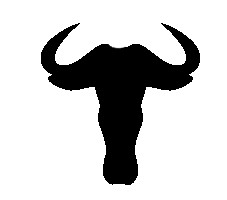
\includegraphics[height=60mm]{13.jpg}} 
&
\frame{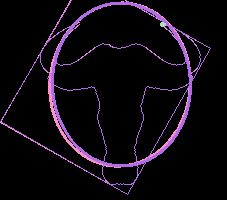
\includegraphics[height=60mm]{13-RectEll.png}}
\\ 
\small  \textbf{تصویر اصلی}  & \small \textbf{تصویر برازش}
\end{tabular}}
\end{center}
 
 
\begin{center}
\makebox[\textwidth]{%
\begin{tabular}{@{}cc@{}}
\frame{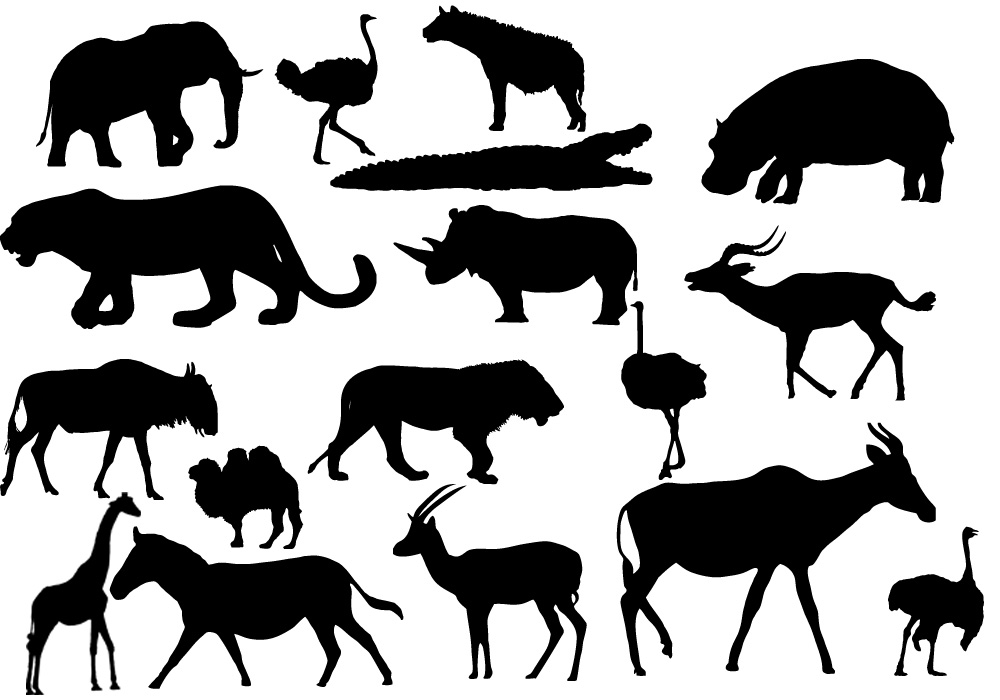
\includegraphics[width=12cm]{african-animals-african-animals-aa-animal-vector.jpg}} 
\\
\small  \textbf{تصویر اصلی} 
\\
\end{tabular}}
\end{center}



\begin{center}
\makebox[\textwidth]{%
\begin{tabular}{@{}cc@{}}
\frame{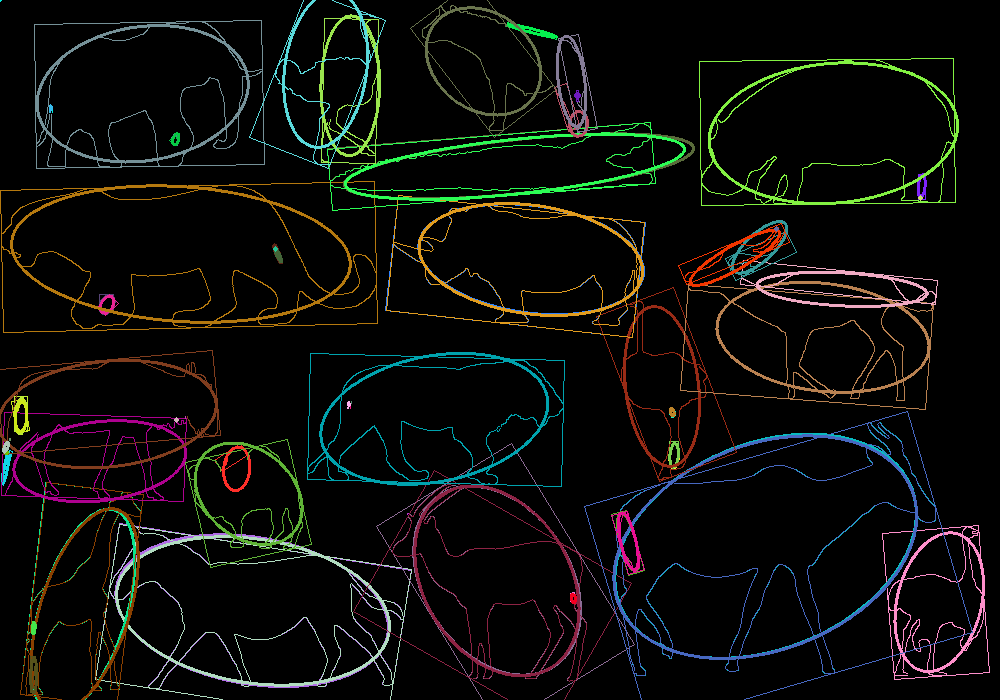
\includegraphics[width=12cm]{african-animals-african-animals-aa-animal-vector-RectEll.png}}
 \\
\small \textbf{تصویر برازش}
\\
\end{tabular}}
\end{center}




\subsection{نازک‌سازی}

\textbf{پرسش:}

 برای محاسبه اسکلت اشیا روش های متعددی وجود دارد. با جستجوی روش ها در اینترنت یکی از این روش ها را با ارائه توضیح مختصر برای انجام تمرین زیر انتخاب کنید. 
 
\textbf{پاسخ:}
روش
\lr{Zhang-Suen}\cite{zhang}
را انتخاب کردیم.
در این روش


\newcommand{\tab}{\hspace*{2em}}
\lr{
    While points are deleted do\\
        \tab For all pixels p(i,j) do\\
           \tab \tab if (a) 2 ≤ B(P1) ≤ 6\\
               \tab \tab \tab(b) A(P1) = 1\\
               \tab \tab \tab(c) Apply one of the following:\\
                  \tab \tab \tab \tab 1. P2 x P4 x P6 = 0 in odd iterations\\
                  \tab \tab \tab \tab 2. P2 x P4 x P8 = 0 in even iterations\\
               \tab \tab \tab (d) Apply one of the following:\\
                  \tab \tab \tab \tab 1. P4 x P6 x P8 = 0 in odd iterations\\
                  \tab \tab \tab \tab 2. P2 x P6 x P8 = 0 in even iterations\\
            \tab \tab \tab then\\
               \tab \tab \tab \tab Delete pixel p(i,j)\\
            \tab \tab \tab end if\\
        \tab \tab  end for\\
    end while\\
}
 
که در آن 
\( A(P_1)\)
تعداد گذر از صفر به یک در همسایگی در جهت ساعت تا 
\( P_9\)
و 
\( B(P_1) \)
تعداد همسایه‌های غیر صفر
\( P_1\)
است. 


\textbf{پرسش:}
 روش ارائه با اسکلت را بر تصویر شماره 12 اعمال کرده و آن را نمایش دهید. این تصویر از ساده ترین نمونه ها برای تشخیص اسکلت است. اگر روش انتخابی شما جواب مناسبی برای این تصویر پیدا نکرد روش را تغییر دهید.
 
\textbf{پاسخ:}

برای این تصویر باید عمل وارون کردن رنگ‌ها صورت گیرد که در رابط کاربری گنجانده‌ شده‌است. نتایج به این شکل شد:


\begin{center}
\makebox[\textwidth]{%
\begin{tabular}{@{}cc@{}}
\frame{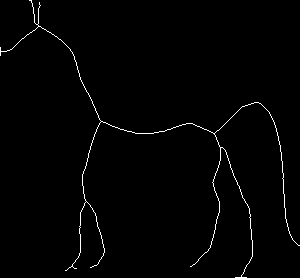
\includegraphics[height=60mm]{12-1-Skel.png}} 
&
\frame{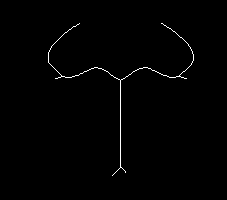
\includegraphics[height=60mm]{13-Skel.png}}
\\ 
\small  \textbf{تصویر ۱۲}  & \small \textbf{تصویر گوزن بخش قبل}
\end{tabular}}
\end{center}
 
 
 
\begin{center}
\makebox[\textwidth]{%
\begin{tabular}{@{}cc@{}}
\frame{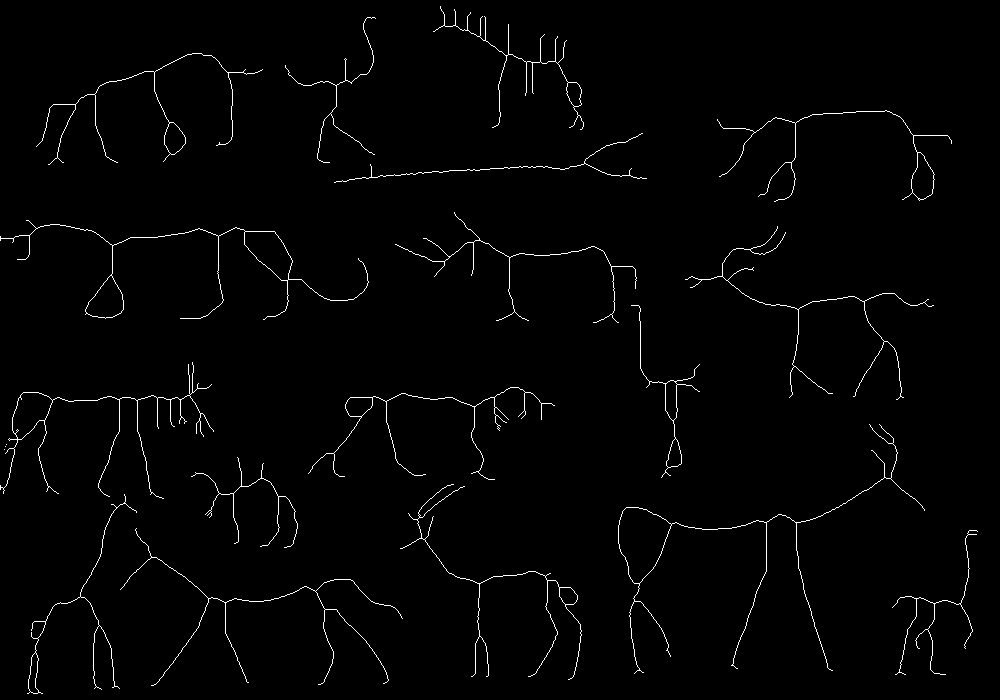
\includegraphics[width=12cm]{african-animals-african-animals-aa-animal-vector-Skel.png}} 
\\
\small  \textbf{تصویر اسکلت حیوانات بخش قبل} 
\\
\end{tabular}}
\end{center}



\textbf{پرسش:}

 برای تصویر 13 و 14 نیز اسکلت شکل را تعیین کنید. آیا با تغییر پارامترهای روش به پاسخ متفاوتی میرسید؟ پاسخ خود را تحلیل کنید.
 
 
\textbf{پاسخ:}

نتایج متفاوت ترشلد کردن اثر گذار است. نتایج در زیر آمده‌است (ترشلد ۱۰۰-۲۵۵) :‌


\begin{center}
\makebox[\textwidth]{%
\begin{tabular}{@{}cc@{}}
\frame{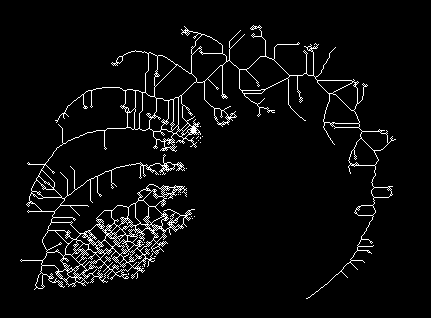
\includegraphics[height=60mm]{15-Skel.png}} 
\\
\small  \textbf{تصویر ۱۳} 
\\
\frame{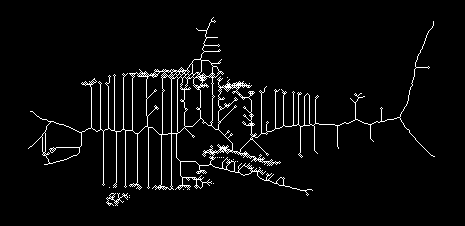
\includegraphics[height=60mm]{14-Skel.png}} 
\\ \small \textbf{تصویر ۱۴}
\\
\end{tabular}}
\end{center}

و نتیجه برای ترشلد بیشتر ۱۰ تا ۲۵۵:


\begin{center}
\makebox[\textwidth]{%
\begin{tabular}{@{}cc@{}}
\frame{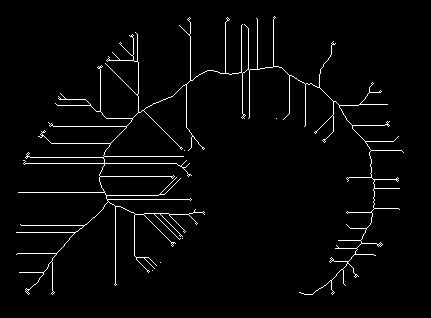
\includegraphics[height=60mm]{215-Skel.png}} 
\\
\small  \textbf{تصویر ۱۳} 
\\
\frame{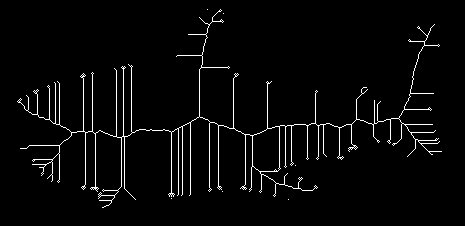
\includegraphics[height=60mm]{214-Skel.png}} 
\\ \small \textbf{تصویر ۱۴}
\\
\end{tabular}}
\end{center}


\begin{center}
\makebox[\textwidth]{%
\begin{tabular}{@{}cc@{}}
\frame{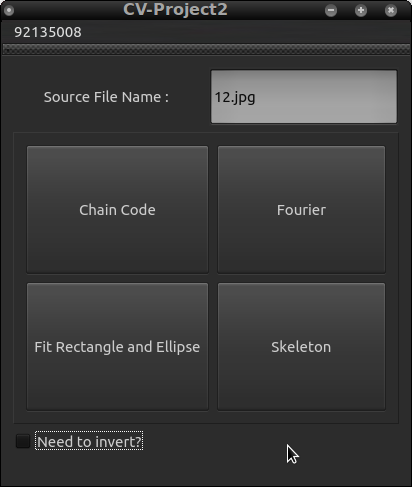
\includegraphics[height=80mm]{main.png}} 
\\
\small  \textbf{نمای نرم‌افزار} 
\\
\end{tabular}}
\end{center}




\newpage




%دستوری برای به حالت عادی درآمدن اندازه فونت‌ها 


\small
%ایجاد «مراجع»


\begin{thebibliography}{99}

\begin{LTRitems}

\resetlatinfont

\bibitem{Hu}
M. Hu, “Visual Pattern Recognition by Moment Invariants,” IRE Transactions on Information Theory, vol. 8, no. 2, pp. 179-187, 1962.

\bibitem{zhang}
T. Y. Zhang,  and C. Y. Suen, “A fast parallel algorithm for thinning digital patterns,” Communications of the ACM, vol. 27, no. 3, pp. 236-239, 1984.

\end{LTRitems}

\end{thebibliography}


\end{document} 
